\section{Menus}
\label{sec:menus}

A menu screen welcomes the player before the actual game starts. This allows
for anything related to setting up a connection with the other device to
happen before the game starts, as well as navigating to different screens.
Since there are no other screens as of right now only a play button is
available.

\subsection{State machine}
\label{sec:state-machine}
To support this mechanic a state machine is implemented. Every screen
corresponds to a state. Every state has an \texttt{enter\_state},
\texttt{execute\_state} and \texttt{exit\_state} function. Upon selecting the
first state the enter function of that state is called once after which the
game loop calls the execute function. Generally the exit function isn't used,
but should the need arise to perform actions upon exiting a state the
possibility is there.

The enter functions are used to perform any necessary initialization as well
as some rendering that only needs to happen once. The execute functions handle
input and perform everything that needs to happen in a gametick.

A simple way to access the states is realised using function pointer arrays.
An enumeration \texttt{game\_state\_t} with all the gamestates is defined in
\texttt{game.h}. Three arrays of function pointers are defined and allocated
in \texttt{game\_state.c}. In that same file the functions for all the states
are defined. The function pointer arrays are then initialized in the same
order the states are defined in \texttt{game\_state\_t}. As a result of all
this all that needs to happen is for a state to be selected using the
\texttt{switch\_state} function. This calls the \texttt{exit\_state} function
of the old state and the \texttt{enter\_state} function of the new state. From
there on \texttt{execute\_current\_state} can be called without actually
having to worry about what state the game is in.

The code supports four different states: a menu screen to welcome the player,
the actual playing state, an endscreen state showing which player won and a
highscores state to list previously set highscores. A diagram is shown below
to illustrate the possible transitions.

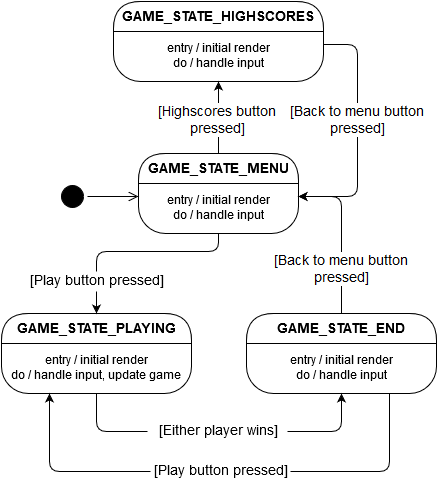
\includegraphics[scale=0.5]{res/state-diagram.png}

There is no code forcing only these transitions to happen, but these are the
only necessary transitions to keep navigation simple.

\subsection{Touch control}
\label{sec:touch-control}
All navigation happens through the touch control in the MI0283QT LCD screen.
The screen is calibrated and touch input is read throug pleasant-lcd from the
pleasant-uno-avr library (see Section~\ref{libraries}).

A struct for buttons is defined in \texttt{touch-buttons.h}. This can be used
to define a button's position and size, as well as an enumeration tag to
identify that button. The file also holds enumerations for the different
buttons in the different screens such as \texttt{touch\_menu\_button\_t}.
These are used for the aforementioned tags to identify buttons.

The actual checking for touch input happens in \texttt{controls.c}. For each
screen that has buttons a different function to process input will have to
be defined. This is so that we're only checking for the buttons actually
available on the screen at any given moment.
